% Options for packages loaded elsewhere
\PassOptionsToPackage{unicode}{hyperref}
\PassOptionsToPackage{hyphens}{url}
\PassOptionsToPackage{dvipsnames,svgnames,x11names}{xcolor}
%
\documentclass[
  11pt,
  a4paper,
]{article}
\usepackage{amsmath,amssymb}
\usepackage{setspace}
\usepackage{iftex}
\ifPDFTeX
  \usepackage[T1]{fontenc}
  \usepackage[utf8]{inputenc}
  \usepackage{textcomp} % provide euro and other symbols
\else % if luatex or xetex
  \usepackage{unicode-math} % this also loads fontspec
  \defaultfontfeatures{Scale=MatchLowercase}
  \defaultfontfeatures[\rmfamily]{Ligatures=TeX,Scale=1}
\fi
\usepackage[]{mathpazo}
\ifPDFTeX\else
  % xetex/luatex font selection
\fi
% Use upquote if available, for straight quotes in verbatim environments
\IfFileExists{upquote.sty}{\usepackage{upquote}}{}
\IfFileExists{microtype.sty}{% use microtype if available
  \usepackage[]{microtype}
  \UseMicrotypeSet[protrusion]{basicmath} % disable protrusion for tt fonts
}{}
\makeatletter
\@ifundefined{KOMAClassName}{% if non-KOMA class
  \IfFileExists{parskip.sty}{%
    \usepackage{parskip}
  }{% else
    \setlength{\parindent}{0pt}
    \setlength{\parskip}{6pt plus 2pt minus 1pt}}
}{% if KOMA class
  \KOMAoptions{parskip=half}}
\makeatother
\usepackage{xcolor}
\usepackage[margin=1in]{geometry}
\usepackage{longtable,booktabs,array}
\usepackage{calc} % for calculating minipage widths
% Correct order of tables after \paragraph or \subparagraph
\usepackage{etoolbox}
\makeatletter
\patchcmd\longtable{\par}{\if@noskipsec\mbox{}\fi\par}{}{}
\makeatother
% Allow footnotes in longtable head/foot
\IfFileExists{footnotehyper.sty}{\usepackage{footnotehyper}}{\usepackage{footnote}}
\makesavenoteenv{longtable}
\usepackage{graphicx}
\makeatletter
\def\maxwidth{\ifdim\Gin@nat@width>\linewidth\linewidth\else\Gin@nat@width\fi}
\def\maxheight{\ifdim\Gin@nat@height>\textheight\textheight\else\Gin@nat@height\fi}
\makeatother
% Scale images if necessary, so that they will not overflow the page
% margins by default, and it is still possible to overwrite the defaults
% using explicit options in \includegraphics[width, height, ...]{}
\setkeys{Gin}{width=\maxwidth,height=\maxheight,keepaspectratio}
% Set default figure placement to htbp
\makeatletter
\def\fps@figure{htbp}
\makeatother
\setlength{\emergencystretch}{3em} % prevent overfull lines
\providecommand{\tightlist}{%
  \setlength{\itemsep}{0pt}\setlength{\parskip}{0pt}}
\setcounter{secnumdepth}{-\maxdimen} % remove section numbering
\pagestyle{plain}
% definitions for citeproc citations
\NewDocumentCommand\citeproctext{}{}
\NewDocumentCommand\citeproc{mm}{%
  \begingroup\def\citeproctext{#2}\cite{#1}\endgroup}
\makeatletter
 % allow citations to break across lines
 \let\@cite@ofmt\@firstofone
 % avoid brackets around text for \cite:
 \def\@biblabel#1{}
 \def\@cite#1#2{{#1\if@tempswa , #2\fi}}
\makeatother
\newlength{\cslhangindent}
\setlength{\cslhangindent}{1.5em}
\newlength{\csllabelwidth}
\setlength{\csllabelwidth}{3em}
\newenvironment{CSLReferences}[2] % #1 hanging-indent, #2 entry-spacing
 {\begin{list}{}{%
  \setlength{\itemindent}{0pt}
  \setlength{\leftmargin}{0pt}
  \setlength{\parsep}{0pt}
  % turn on hanging indent if param 1 is 1
  \ifodd #1
   \setlength{\leftmargin}{\cslhangindent}
   \setlength{\itemindent}{-1\cslhangindent}
  \fi
  % set entry spacing
  \setlength{\itemsep}{#2\baselineskip}}}
 {\end{list}}
\usepackage{calc}
\newcommand{\CSLBlock}[1]{\hfill\break\parbox[t]{\linewidth}{\strut\ignorespaces#1\strut}}
\newcommand{\CSLLeftMargin}[1]{\parbox[t]{\csllabelwidth}{\strut#1\strut}}
\newcommand{\CSLRightInline}[1]{\parbox[t]{\linewidth - \csllabelwidth}{\strut#1\strut}}
\newcommand{\CSLIndent}[1]{\hspace{\cslhangindent}#1}
\usepackage{lineno} % add 
\usepackage{amsmath} % add 
\linenumbers % turns line numbering on 

% Allowing for landscape pages
\usepackage{lscape}
\newcommand{\blandscape}{\begin{landscape}}
\newcommand{\elandscape}{\end{landscape}}

% Left justification of the text: see https://www.sharelatex.com/learn/Text_alignment
% \usepackage[document]{ragged2e} % already in the latex template
\newcommand{\bleft}{\begin{flushleft}}
\newcommand{\eleft}{\end{flushleft}}


% Add Supplementary Tables and Figures
% Code from https://stackoverflow.com/a/51337664
\newcommand{\beginsupplement}{
  \setcounter{table}{0}  
  \renewcommand{\thetable}{S\arabic{table}}
  \setcounter{figure}{0} 
  \renewcommand{\thefigure}{S\arabic{figure}}
}



\ifLuaTeX
  \usepackage{selnolig}  % disable illegal ligatures
\fi
\usepackage{bookmark}
\IfFileExists{xurl.sty}{\usepackage{xurl}}{} % add URL line breaks if available
\urlstyle{same}
\hypersetup{
  pdftitle={Spatial occupancy models for data collected on stream networks},
  pdfauthor={Olivier Gimenez1*},
  colorlinks=true,
  linkcolor={RoyalBlue},
  filecolor={Maroon},
  citecolor={Blue},
  urlcolor={RoyalBlue},
  pdfcreator={LaTeX via pandoc}}

\title{Spatial occupancy models for data collected on stream networks}
\author{Olivier Gimenez\textsuperscript{1}*}
\date{2024-07-25}

\begin{document}
\maketitle

\setstretch{2}
\small

\textsuperscript{1} CEFE, Univ Montpellier, CNRS, EPHE, IRD, Montpellier, France

\texttt{*} Corresponding author: \href{mailto:olivier.gimenez@cefe.cnrs.fr}{\nolinkurl{olivier.gimenez@cefe.cnrs.fr}}

\normalsize

\vspace{1cm}
\hrule

To monitor streams and rivers biodiversity, we need to quantify species distribution. To do so, occupancy models allow distinguishing the non-detection of a species from its actual absence. Occupancy models can account for spatial autocorrelation, but are not suited for streams and rivers because of their spatial structure in networks. Here I propose spatial occupancy models for data collected on stream and river networks. I present the statistical developments of the model, then I illustrate the approach on a semi-aquatic mammal. Overall, spatial stream network occupancy models provide a formal approach to assess biodiversity in streams and rivers.

\vspace{3mm}
\hrule
\vspace{5mm}

\emph{Keywords}: Bayesian statistics, Spatial stream network models, Occupancy models, Spatial autocorrelation, Wildlife monitoring

\bleft
\newpage

\section{Introduction}\label{introduction}

Streams and rivers provide essential habitats for numerous species of animals and plants, many of which are endemic (\citeproc{ref-D2006}{Dudgeon et al. 2006}, \citeproc{ref-Reid2019}{Reid et al. 2019}). The ecological health of these freshwater ecosystems is paramount not only for the biodiversity they harbor but also for the ecosystem services they provide, which are indispensable to both wildlife and human populations (\citeproc{ref-V2022}{Vári et al. 2021}). However, human activities are altering the natural conditions of streams, rivers and their associated riparian habitats, jeopardizing the persistence of these ecosystems (\citeproc{ref-A2020}{Albert et al. 2020}).

In that context, species distribution models (SDMs) are essential tools in understanding and preserving biodiversity (\citeproc{ref-Elith2009}{Elith and Leathwick 2009}). SDMs predict the distribution of species, helping scientists and conservationists identify critical habitats and biodiversity hotspots. SDMs also inform strategies aimed at mitigating impacts of climate and land-use changes, manage invasive species or enhancing habitat connectivity in freshwater ecosystems (\citeproc{ref-D2015}{Domisch et al. 2015}).

SDMs are known to be affected by two main issues, namely imperfect detection and spatial autocorrelation (\citeproc{ref-GK2018}{Guélat and Kéry 2018}). First, a species present in a given area may go undetected during surveys due to various factors such as observer experience, species behavior, and environmental conditions. Ignoring \emph{imperfect detection} can lead to biased estimates of species distribution, and flawed inference about the relationship between species presence and environmental factors (\citeproc{ref-Kery2008}{Kéry and Schmidt 2008}, \citeproc{ref-Lahoz2014}{Lahoz-Monfort et al. 2014}), potentially misinforming conservation strategies and habitat management decisions. To address this issue, occupancy models are SDMs that rely on repeated visits of spatial sampling units for inferring distribution (\citeproc{ref-mackenzie2017}{MacKenzie et al. 2017}). These models have been widely used in freshwater ecosystems for various taxa (\citeproc{ref-Hamer2021}{Hamer et al. 2021}, \citeproc{ref-Preece2021}{Preece et al. 2021}, \citeproc{ref-Charbonnel2022}{Charbonnel et al. 2022}, \citeproc{ref-Wedderburn2022}{Wedderburn et al. 2022}). Second, SDMs rely on the assumption of independent residuals, which may be violated if sampling sites that are close together tend to have similar probabilities of species presence. Ignoring \emph{spatial autocorrelation} can lead to biased estimates of species distribution, and can inflate the probability of erroneously detecting the effect of environmental covariates (\citeproc{ref-Dormann2007}{Dormann et al. 2007}). Several extensions of occupancy models have been proposed to account for spatial autocorrelation, building on the spatial statistics literature, e.g.~conditional autoregressive models (\citeproc{ref-Johnson2013}{Johnson et al. 2013}, \citeproc{ref-Broms2014}{Broms et al. 2014}) and geoadditive models (\citeproc{ref-Rushing2019}{Rushing et al. 2019}). However, these models rely on the Euclidean distance between the spatial sampling units, which does not acknowledge the spatial structure in networks of streams and rivers.

Here I propose spatial occupancy models that allow spatial autocorrelation structured according to stream flow and flow connectivity (\citeproc{ref-Peterson2013}{Peterson et al. 2013}). I build on the linear mixed modelling approach proposed by (\citeproc{ref-Peterson2010}{Peterson and Hoef 2010}, \citeproc{ref-VerHoef2010}{Ver Hoef and Peterson 2010}), which allows considering a mixture of distance-based spatial correlation structures (Euclidean or not) in a single model. I plug-in this variance component approach into occupancy models using a Bayesian approach. I present the statistical developments of the model, and I illustrate the approach on a semi-aquatic mammal in French streams and rivers.

\section{Methods}\label{methods}

\subsection{Occupancy models}\label{occupancy-models}

To account for imperfect detection, I use occupancy models that allow inferring the actual species distribution (\citeproc{ref-mackenzie2017}{MacKenzie et al. 2017}). We assume the monitoring of a species occurs over \(S\) spatial sampling units, or \emph{sites}. If detection was perfect, the state \(z_i\) of a site \(i\) would be a Bernoulli random variable taking value 1 with \emph{occupancy probability} \(\psi_i\) if the site was occupied, and 0 otherwise with probability \(1-\psi\). However, the ecological process of state occupancy \(z_i\) is only partially known, because the species may go undetected whereas actually present of that site \(i\). Therefore we need to consider the observation process, also a Bernoulli random variable, on top of the ecological process. When the species is detected on site \(i\), say \(y_i = 1\) with \emph{detection probability} \(p\), then that site is occupied, whereas if the species goes undetected with probability \(1-p\), i.e.~\(y_i = 0\), we simply do not know whether the site is occupied or not. Both parameters, \(\psi\) and \(p\), can be modeled as functions of explanatory spatial variables, in the spirit of generalized linear models and logistic regressions. The only requirement to separately estimate the occupancy and detection probabilities is to collect data in at least two independent visits in time for a number of sites, and this temporal replication should be over a short period so that sites remain in the same state.

\subsection{Spatial autocorrelation for stream networks}\label{spatial-autocorrelation-for-stream-networks}

How is spatial autocorrelation accounted for in occupancy models? The usual way is to write the probabilities of occupancy \(\boldsymbol{\psi} = (\psi_1, \ldots, \psi_S)\) on some scale, say the logit scale, as a function of explanatory variables gathered in a matrix \(\mathbf{X}\) with corresponding regression parameters \(\boldsymbol{\beta}\) to be estimated, and add a random effect \(\boldsymbol{\epsilon}\) to capture spatial autocorrelation (\citeproc{ref-GK2018}{Guélat and Kéry 2018}):

\begin{equation*}
\text{logit}(\boldsymbol{\psi}) = \mathbf{X} \boldsymbol{\beta} + \boldsymbol{\epsilon}.
\end{equation*}

The random effect \(\boldsymbol{\epsilon}\) can be structured using a conditional autoregressive models and its extensions (\citeproc{ref-Johnson2013}{Johnson et al. 2013}) or geoadditive models (\citeproc{ref-Rushing2019}{Rushing et al. 2019}). Whatever the method, the proximity among sites is assessed using the Euclidean distance, which fails to adequately capture complex spatial dependencies in streams and rivers. Specifically, we are interested in flow connectivity and stream and river topology (\citeproc{ref-Peterson2013}{Peterson et al. 2013}). Following (\citeproc{ref-Peterson2010}{Peterson and Hoef 2010}, \citeproc{ref-VerHoef2010}{Ver Hoef and Peterson 2010}), I consider two sites as being \emph{flow-connected} when water flows from an upstream site to a downstream site, and \emph{flow-unconnected} when they share a common confluence downstream but do not share flow. Then I parameterize occupancy by rewriting the random effect as a mixture of four components as follows:

\begin{equation*}
\text{logit}(\boldsymbol{\psi}) = \mathbf{X} \boldsymbol{\beta} + \boldsymbol{\tau}_{tu} + \boldsymbol{\tau}_{td} + \boldsymbol{\tau}_{eu} + \boldsymbol{\epsilon}
\end{equation*}

where \(\boldsymbol{\tau}_{tu}\) is a random effect with spatial covariance between flow-connected sites that can occur in the same direction of the river flow (\emph{tail-up}, think of organisms that move passively like, e.g., mussels), \(\boldsymbol{\tau}_{td}\) is a random effect with spatial covariance between flow-connected and flow-unconnected sites that can occur with or against the direction of the flow (\emph{tail-down}, think of organisms that move actively like, e.g., semi-aquatic mammals), \(\boldsymbol{\tau}_{eu}\) is a random effect with a spatial covariance independent of the network topology (generated by, e.g., air temperature or precipitation), and \(\boldsymbol{\epsilon}\) is a random effect which variance, often called the nugget, can absorb extra-variability. Writing these covariance components is described in details elsewhere: Appendix B in (\citeproc{ref-Peterson2010}{Peterson and Hoef 2010}), (\citeproc{ref-isaak2014applications}{Isaak et al. 2014}). I provide an example below.

\subsection{Implementation}\label{implementation}

For all analyses, I used the statistical language \texttt{R} (\citeproc{ref-R_Core_Team_2023}{R Core Team 2023}). I fitted models in the Bayesian framework by specifying weakly informative priors (\citeproc{ref-Northrup2018}{Northrup and Gerber 2018}), implementing a marginalized likelihood (\citeproc{ref-clark2019}{Clark and Altwegg 2019}) and using the \texttt{rstan} (\citeproc{ref-Stan_Development_Team_2023}{Stan Development Team 2023}) package. I also used the \texttt{openSTARS} (\citeproc{ref-Kattwinkel2020}{Kattwinkel et al. 2020}) and \texttt{SSN} (\citeproc{ref-VerHoef2014}{Hoef et al. 2014}) packages to build and characterize the network and calculate hydrological distances.

\subsection{Case study}\label{case-study}

(\citeproc{ref-Couturier2024}{Couturier et al. 2023})

(\citeproc{ref-Kervellec2023}{Kervellec et al. 2023})

Sites in counties Lot (46), Aveyron (12) and Cantal (15). First two are in Pyrénées, third is in Massif Central.

The species went almost extinct in the 20th century, it was hunted for its fur. Thanks to the banning of hunting and its protection, it is now recolonizing our country. In that context, the question we're asking is what is its current distribution.

To answer this question, we collect scats the species leaves behind.

Now to the case study. I investigated the effect of human disturbance on otter occupancy.
The study site is in this rectangle here, between Montpellier where I live and Swansea.
There were 56 sites that were visited 3 times.
Clearly we have some spatial variation in the number of detections.
I used human density as a proxy for human disturbance.
Human density can lead to disturbance of otters through urbanization for example.
We recorded human density as the number of inhabitants per km2 in a buffer around each stream.

I use tail-down only. Exponential structure, with decreasing correlation with increasing distance. Ecrire le modèle ici avec l'exponentielle:

\[
    \text{Cov}(\epsilon_i,\epsilon_j)= 
\begin{cases}
    \displaystyle{\sigma^2\exp(-d_{ij}/\theta)},& \text{if sites } i \text{ and } j \text{ are connected }\\
    0,              & \text{otherwise}
\end{cases}
\]

Expliquer les paramètres d, s et theta.

\section{Results}\label{results}

See Fig. \ref{fig:mainfig}.

When spatial autocorrelation is ignored, we found a negative effect of human density on occupancy probability.

However, when we accounted for spatial autocorrelation using our new model, human density had no longer an effect on occupancy.

The effect size of human density increases when spatial autocorrelation is ignored.

The most likely explanation is that of a bias due to an omitted variable.
Human density is spatially correlated, and its effect size is inflated.
This bias is controlled when spatial autocorrelation is included.
There is probably a difference in occupancy according to another variable that would need to be accounted for.

\section{Discussion}\label{discussion}

Si besoin, merge results and discussion sections.

The focal ecological parameter of interest is the occupancy probability \(\psi\), which is represented similarly in all the five models compared. However, the precision of the occupancy estimation is impacted by the quality of the estimation for the detection process (kery2008, kellner2014). In this study, we focused on cases in which data is collected continuously, for example with sensors or opportunistic data. We aimed to evaluate whether modelling the detection process in continuous time could enhance the precision of the estimated probability of occupancy.

Ecologically, omitted bias variable. Check in Couturier which one it could be. Citer quand même le papier de Hodges sur spatial confusion. Citer aussi les échanges avec Jay VerHoef pour la difficulté in estimating le sill parameter. Mais ok pour covariate et prediction de l'occupancy.

Application à eDNA. Alors besoin peut-être d'autres termes spatiaux comme tail-up, et euclidean. Ici on a utilisé que tail-down car on s'interesse aux otters. eDNA important pour monitor biodiv in freshwater and marine realms. If false positives wored out (voir work de E. Matechou), resste à proprement prendfre en compte spatial autocorrelation.

Extension à dynamic occupancy models. Colonization function of distance to features that hamper movement of individuals. Citer les papier de Chandler, Morin et celui à paraître de Kervellec. L'idée est qu'on pourrait regarder la question de la connectivité dans river et stream network. Pas super compliqué, le papier du portuguais a paved the road.

Extending to dynamic occupancy to write the probability of colonization as a function of distance to landscape features that might hamper movements, and therefore assessing connectivity.

From paper by Johnson. By exploiting autocorrelation when present, one can potentially decrease the number of visits to specific survey units
within a study area, instead relying on spatial dependence to take the place of some temporal replication.
ALSO. The issue of spatial confounding is relatively new in
the statistics literature. As Hodges and Reich (2010)
state, it is a ``rich area of research.'\,' Experienced spatial
modelers might say that confounding is desirable as it
allows an adjustment in fixed effects inference due to
unmeasured (unknown), spatially correlated covariates.
However, Hodges, Hodges and Reich (2010) and
Paciorek (2010) illustrate bias and variance inflation
depend on the structure of these unmeasured variables.
Because the structure of these latent spatial variables is
unknown, a spatial model may not account for them the
way the researcher intends. Hodges and Reich (2010)
note that without knowledge of the missing structure,
purposefully adding spatial confounding is a haphazard
adjustment that may bias the known fixed effects in
unknown ways. There may be some middle ground,
however, that is worth exploring (Paciorek 2010) and
could be the topic of future research in the context of
occupancy modeling and spatial modeling in general.

From Rushing paper. The distributions of most species are characterized by complex and dynamic variation in occurrence. Species distribution modeling seeks to relate this variation to environmental covariates and extrapolate these relationships to unsampled sites and times. Because habitats and species-habitat relationships change across both space and time, conventional GLM-based models rarely capture the inherent complexity of species distributions, especially when inferences are made across large spatial or long temporal scales. Here, we demonstrate a novel occupancy-based SDM that combines environmental predictors with a spatial GAM to model covariate relationships and complex, non-linear spatial variation in occupancy probability while accounting for imperfect detection.

Acknowledge similar approach for count data by (\citeproc{ref-Lu2024}{Lu et al. 2024}).

\section{Acknowledgments}\label{acknowledgments}

Jay Ver Hoef, Edgar Santos Fernández and Maëlis Kervellec.

\section{Ethics and Integrity statements}\label{ethics-and-integrity-statements}

\subsection{Data availability statement}\label{data-availability-statement}

Data and code are available at \href{https://github.com/oliviergimenez/spatial-stream-network-occupancy-model}{https://github.com/oliviergimenez/spatial-stream-network-occupancy-model}.

\subsection{Funding statement}\label{funding-statement}

This research is a product of the DISCAR group funded by the French Foundation for Research on Biodiversity (FRB) through its synthesis center CESAB.

\subsection{Conflict of interest disclosure}\label{conflict-of-interest-disclosure}

The author has no conflicts of interest to declare.

\section{References}\label{references}

\phantomsection\label{refs}
\begin{CSLReferences}{1}{0}
\bibitem[\citeproctext]{ref-A2020}
Albert, J. S., G. Destouni, S. M. Duke-Sylvester, A. E. Magurran, T. Oberdorff, R. E. Reis, K. O. Winemiller, and W. J. Ripple. 2020. Scientists' warning to humanity on the freshwater biodiversity crisis. Ambio 50:85--94.

\bibitem[\citeproctext]{ref-Broms2014}
Broms, K. M., D. S. Johnson, R. Altwegg, and L. L. Conquest. 2014. Spatial occupancy models applied to atlas data show southern ground hornbills strongly depend on protected areas. Ecological Applications 24:363--374.

\bibitem[\citeproctext]{ref-Charbonnel2022}
Charbonnel, A., F. Blanc, P. Laffaille, M. Némoz, and L. Buisson. 2022. Combining spatial dependence occupancy models and conservation gap analyses to promote species conservation: A case study with a threatened semi-aquatic mammal. Biological Conservation 270:109567.

\bibitem[\citeproctext]{ref-clark2019}
Clark, A. E., and R. Altwegg. 2019. Efficient {B}ayesian analysis of occupancy models with logit link functions. Ecology and Evolution 9:756--768.

\bibitem[\citeproctext]{ref-Couturier2024}
Couturier, T., J. Steinmetz, P. Defos du Rau, D. Marc, E. Trichet, R. Gomes, and A. Besnard. 2023. Intensive agriculture as the main limiting factor of the otter's return in southwest france. Biological Conservation 279:109927.

\bibitem[\citeproctext]{ref-D2015}
Domisch, S., S. Jähnig, J. Simaika, M. Kuemmerlen, and S. Stoll. 2015. Application of species distribution models in stream ecosystems: The challenges of spatial and temporal scale, environmental predictors and species occurrence data. Fundamental and Applied Limnology 186:45--61.

\bibitem[\citeproctext]{ref-Dormann2007}
Dormann, F. C., J. M. McPherson, M. B. Araújo, R. Bivand, J. Bolliger, G. Carl, R. G. Davies, A. Hirzel, W. Jetz, W. Daniel Kissling, I. Kühn, R. Ohlemüller, P. R. Peres-Neto, B. Reineking, B. Schröder, F. M. Schurr, and R. Wilson. 2007. Methods to account for spatial autocorrelation in the analysis of species distributional data: A review. Ecography 30:609--628.

\bibitem[\citeproctext]{ref-D2006}
Dudgeon, D., A. H. Arthington, M. O. Gessner, Z.-I. Kawabata, D. J. Knowler, C. Lévêque, R. J. Naiman, A.-H. Prieur-Richard, D. Soto, M. L. J. Stiassny, and C. A. Sullivan. 2006. Freshwater biodiversity: Importance, threats, status and conservation challenges. Biological Reviews 81:163--182.

\bibitem[\citeproctext]{ref-Elith2009}
Elith, J., and J. R. Leathwick. 2009. Species distribution models: Ecological explanation and prediction across space and time. Annual Review of Ecology, Evolution, and Systematics 40:677--697.

\bibitem[\citeproctext]{ref-GK2018}
Guélat, J., and M. Kéry. 2018. Effects of spatial autocorrelation and imperfect detection on species distribution models. Methods in Ecology and Evolution 9:1614--1625.

\bibitem[\citeproctext]{ref-Hamer2021}
Hamer, A. J., D. Schmera, and M. J. Mahony. 2021. Multi-species occupancy modeling provides novel insights into amphibian metacommunity structure and wetland restoration. Ecological Applications 31:e2293.

\bibitem[\citeproctext]{ref-VerHoef2014}
Hoef, J. M. V., E. E. Peterson, D. Clifford, and R. Shah. 2014. {SSN}: An {R} package for spatial statistical modeling on stream networks. Journal of Statistical Software 56:1--45.

\bibitem[\citeproctext]{ref-isaak2014applications}
Isaak, D. J., E. E. Peterson, J. M. Ver Hoef, S. J. Wenger, J. A. Falke, C. E. Torgersen, C. Sowder, E. A. Steel, M.-J. Fortin, C. E. Jordan, and others. 2014. Applications of spatial statistical network models to stream data. Wiley Interdisciplinary Reviews: Water 1:277--294.

\bibitem[\citeproctext]{ref-Johnson2013}
Johnson, D. S., P. B. Conn, M. B. Hooten, J. C. Ray, and B. A. Pond. 2013. Spatial occupancy models for large data sets. Ecology 94:801--808.

\bibitem[\citeproctext]{ref-Kattwinkel2020}
Kattwinkel, M., E. Szöcs, E. Peterson, and R. Schäfer. 2020. Preparing GIS data for analysis of stream monitoring data: The {R} package openSTARS. Plos One 15:e0239237.

\bibitem[\citeproctext]{ref-Kervellec2023}
Kervellec, M., T. Couturier, S. Bauduin, D. Chenesseau, P. D. du Rau, N. Drouet-Hoguet, C. Duchamp, J. Steinmetz, J.-M. Vandel, and O. Gimenez. 2023. Bringing circuit theory into spatial occupancy models to assess landscape connectivity. bioRxiv.

\bibitem[\citeproctext]{ref-Kery2008}
Kéry, M., and B. Schmidt. 2008. Imperfect detection and its consequences for monitoring in conservation. Community Ecology 9:207--216.

\bibitem[\citeproctext]{ref-Lahoz2014}
Lahoz-Monfort, J. J., G. Guillera-Arroita, and B. A. Wintle. 2014. Imperfect detection impacts the performance of species distribution models. Global Ecology and Biogeography 23:504--515.

\bibitem[\citeproctext]{ref-Lu2024}
Lu, X., Y. Kanno, G. P. Valentine, J. M. Rash, and M. B. Hooten. 2024. Using multi-scale spatial models of dendritic ecosystems to infer abundance of a stream salmonid. Journal of Applied Ecology 61:1703--1715.

\bibitem[\citeproctext]{ref-mackenzie2017}
MacKenzie, D. I., J. D. Nichols, J. A. Royle, K. H. Pollock, L. L. Bailey, and J. E. Hines. 2017. Occupancy {Estimation} and {Modeling}: {Inferring Patterns} and {Dynamics} of {Species Occurrence}. {Elsevier}.

\bibitem[\citeproctext]{ref-Northrup2018}
Northrup, J., and B. Gerber. 2018. A comment on priors for {B}ayesian occupancy models. Plos One 13:e0192819.

\bibitem[\citeproctext]{ref-Peterson2010}
Peterson, E. E., and J. M. V. Hoef. 2010. A mixed-model moving-average approach to geostatistical modeling in stream networks. Ecology 91:644--651.

\bibitem[\citeproctext]{ref-Peterson2013}
Peterson, E. E., J. M. Ver Hoef, D. J. Isaak, J. A. Falke, M.-J. Fortin, C. E. Jordan, K. McNyset, P. Monestiez, A. S. Ruesch, A. Sengupta, N. Som, E. A. Steel, D. M. Theobald, C. E. Torgersen, and S. J. Wenger. 2013. Modelling dendritic ecological networks in space: An integrated network perspective. Ecology Letters 16:707--719.

\bibitem[\citeproctext]{ref-Preece2021}
Preece, E. P., M. Bryan, S. M. Mapes, C. Wademan, and R. Dorazio. 2021. Monitoring for freshwater mussel presence in rivers using environmental DNA. Environmental DNA 3:591--604.

\bibitem[\citeproctext]{ref-R_Core_Team_2023}
R Core Team. 2023. \href{https://www.R-project.org/}{R: A language and environment for statistical computing}. R Foundation for Statistical Computing, Vienna, Austria.

\bibitem[\citeproctext]{ref-Reid2019}
Reid, A. J., A. K. Carlson, I. F. Creed, E. J. Eliason, P. A. Gell, P. T. J. Johnson, K. A. Kidd, T. J. MacCormack, J. D. Olden, S. J. Ormerod, J. P. Smol, W. W. Taylor, K. Tockner, J. C. Vermaire, D. Dudgeon, and S. J. Cooke. 2019. Emerging threats and persistent conservation challenges for freshwater biodiversity. Biological Reviews 94:849--873.

\bibitem[\citeproctext]{ref-Rushing2019}
Rushing, C., J. andrew Royle, D. Ziolkowski Jr, and K. Pardieck. 2019. Modeling spatially and temporally complex range dynamics when detection is imperfect. Scientific Reports 9.

\bibitem[\citeproctext]{ref-Stan_Development_Team_2023}
Stan Development Team. 2023. \href{https://mc-stan.org/}{{RStan}: The {R} interface to {Stan}}.

\bibitem[\citeproctext]{ref-V2022}
Vári, Á., S. Podschun, T. Eros, T. Hein, B. Pataki, C. Ioja, C. Adamescu, A. Gerhardt, T. Gruber, A. Dedić, M. Ciric, B. Gavrilović, and A. Báldi. 2021. Freshwater systems and ecosystem services: Challenges and chances for cross-fertilization of disciplines. Ambio 51:135--151.

\bibitem[\citeproctext]{ref-VerHoef2010}
Ver Hoef, J., and E. Peterson. 2010. A moving average approach for spatial statistical models of stream networks. Journal of the American Statistical Association 105:6--18.

\bibitem[\citeproctext]{ref-Wedderburn2022}
Wedderburn, S. D., N. S. Whiterod, and L. Vilizzi. 2022. Occupancy modelling confirms the first extirpation of a freshwater fish from one of the world's largest river systems. Aquatic Conservation: Marine and Freshwater Ecosystems 32:258--268.

\end{CSLReferences}

\eleft

\clearpage

\newpage

\blandscape

\begin{figure}[b]

{\centering 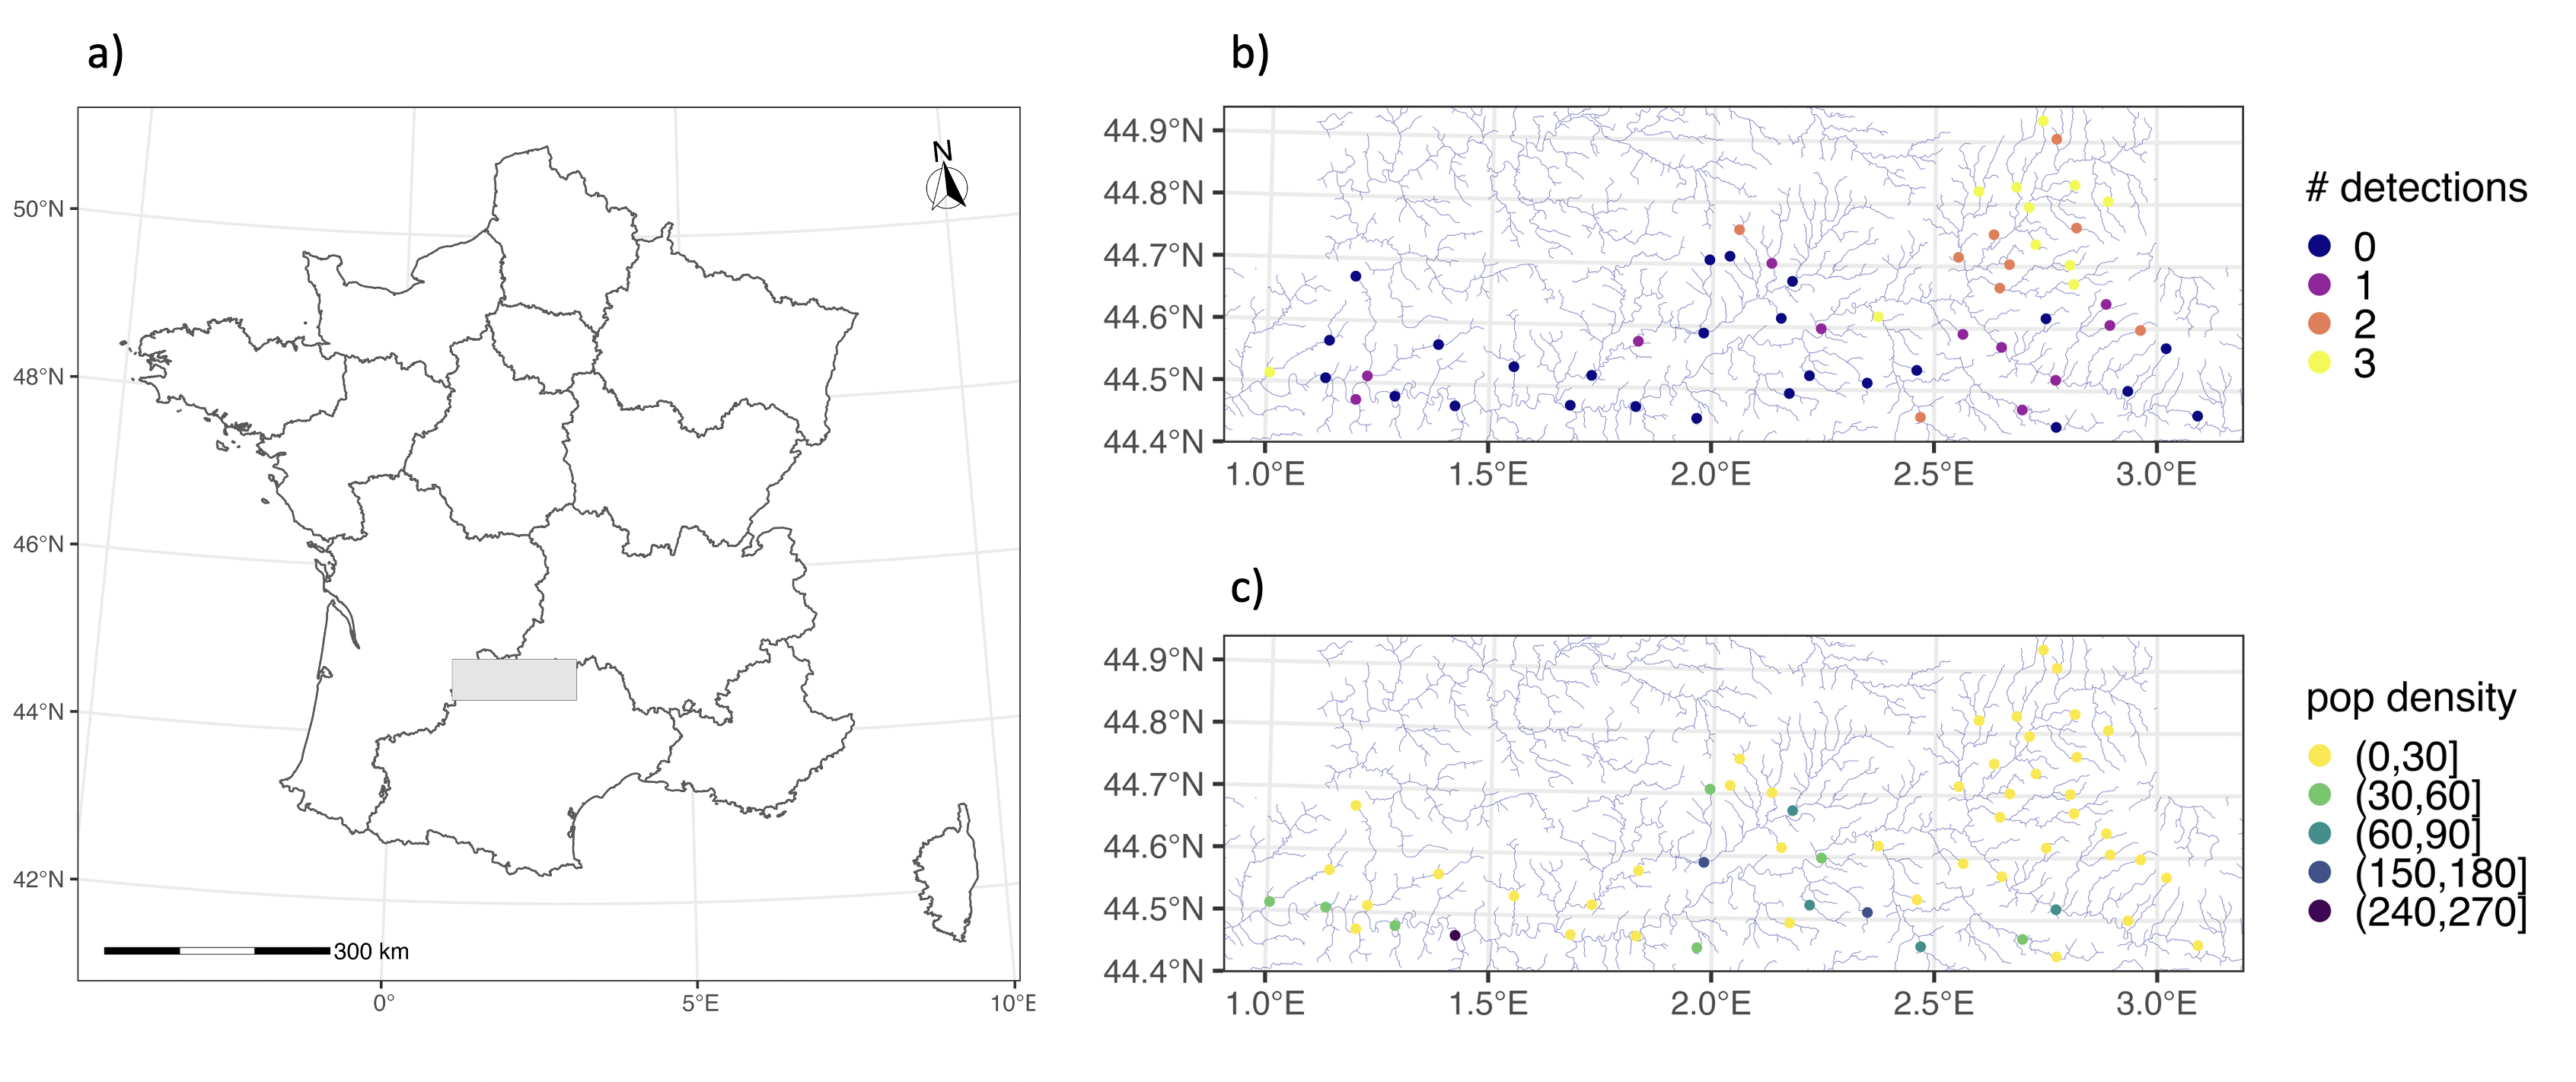
\includegraphics[width=0.98\linewidth]{mainfigure} 

}

\caption{Second figure in landscape format.}\label{fig:mainfig}
\end{figure}

\elandscape

\end{document}
